\documentclass{beamer}
\usepackage{beamerthemesplit}
\usepackage{graphics}
\logo{\includegraphics[height=1cm]{psi_logo_white.png}}
\usetheme{Pittsburgh}
\usecolortheme{dove}
\beamertemplatenavigationsymbolsempty
\setbeamertemplate{footline}[frame number]
\definecolor{myback}{RGB}{175,238,238}
\setbeamercolor{structure}{bg=myback}
\usepackage[T1]{fontenc}
\newcommand{\changefont}[3] {
 \fontfamily{#1} \fontseries{#2} \fontshape{#3} \selectfont}

\title{NeXus and PHDF}
\author{Mark K\"onnecke }
\institute{Paul Scherrer Institute\\Switzerland }
\date{\today} 

\begin{document}

%%\begin{frame}
%%\titlepage
%% \end{frame}


\begin{frame} \frametitle{Minimum}
\begin{tabbing}
\hspace*{1cm} \= \hspace*{1cm} \= \hspace*{1cm} \= \hspace*{1cm} \= \hspace*{1cm} \= \hspace*{1cm}\= \kill
entry:NXDetector \\
  \>data[NP,xsize,ysize], signal=1 (1)\\
  \>further detetcor parameters, using NeXus names where possible\\
\end{tabbing}
\begin{itemize}
\item Programming model:
\begin{itemize}
\item Dectris writes frames in HDF-5
\item Institute DAQ writes metadata, creates structures
\item Links internally or externally to detector data
\end{itemize}
\item Performance: near raw disk I/O when using large chunks
\end{itemize}
\end{frame}

\begin{frame} \frametitle{More}
\begin{tabbing}
\hspace*{1cm} \= \hspace*{1cm} \= \hspace*{1cm} \= \hspace*{1cm} \= \hspace*{1cm} \= \hspace*{1cm}\= \kill
entry:NXentry \\
 \>instrument:NXinstrument\\
 \> \> detector:NXdetector \\
 \> \> \>data[NP,xsize,ysize], signal=1 (1)\\
 \> \> \>further detetcor parameters, using NeXus names where possible\\
\end{tabbing}
\end{frame}

\begin{frame}
\frametitle{More Wishes}
\begin{itemize}
\item Diamond: data[nx,ny,xdim,ydim] for 2D scans
\item APS: Rather a library then Camserver
\item APS: latency of writing/reading file to much
\end{itemize}
\end{frame}


\end{document}

\begin{frame} \frametitle{NeXus Simple Coordinate System }
\begin{figure}[!ht]
\resizebox{7cm}{5cm}{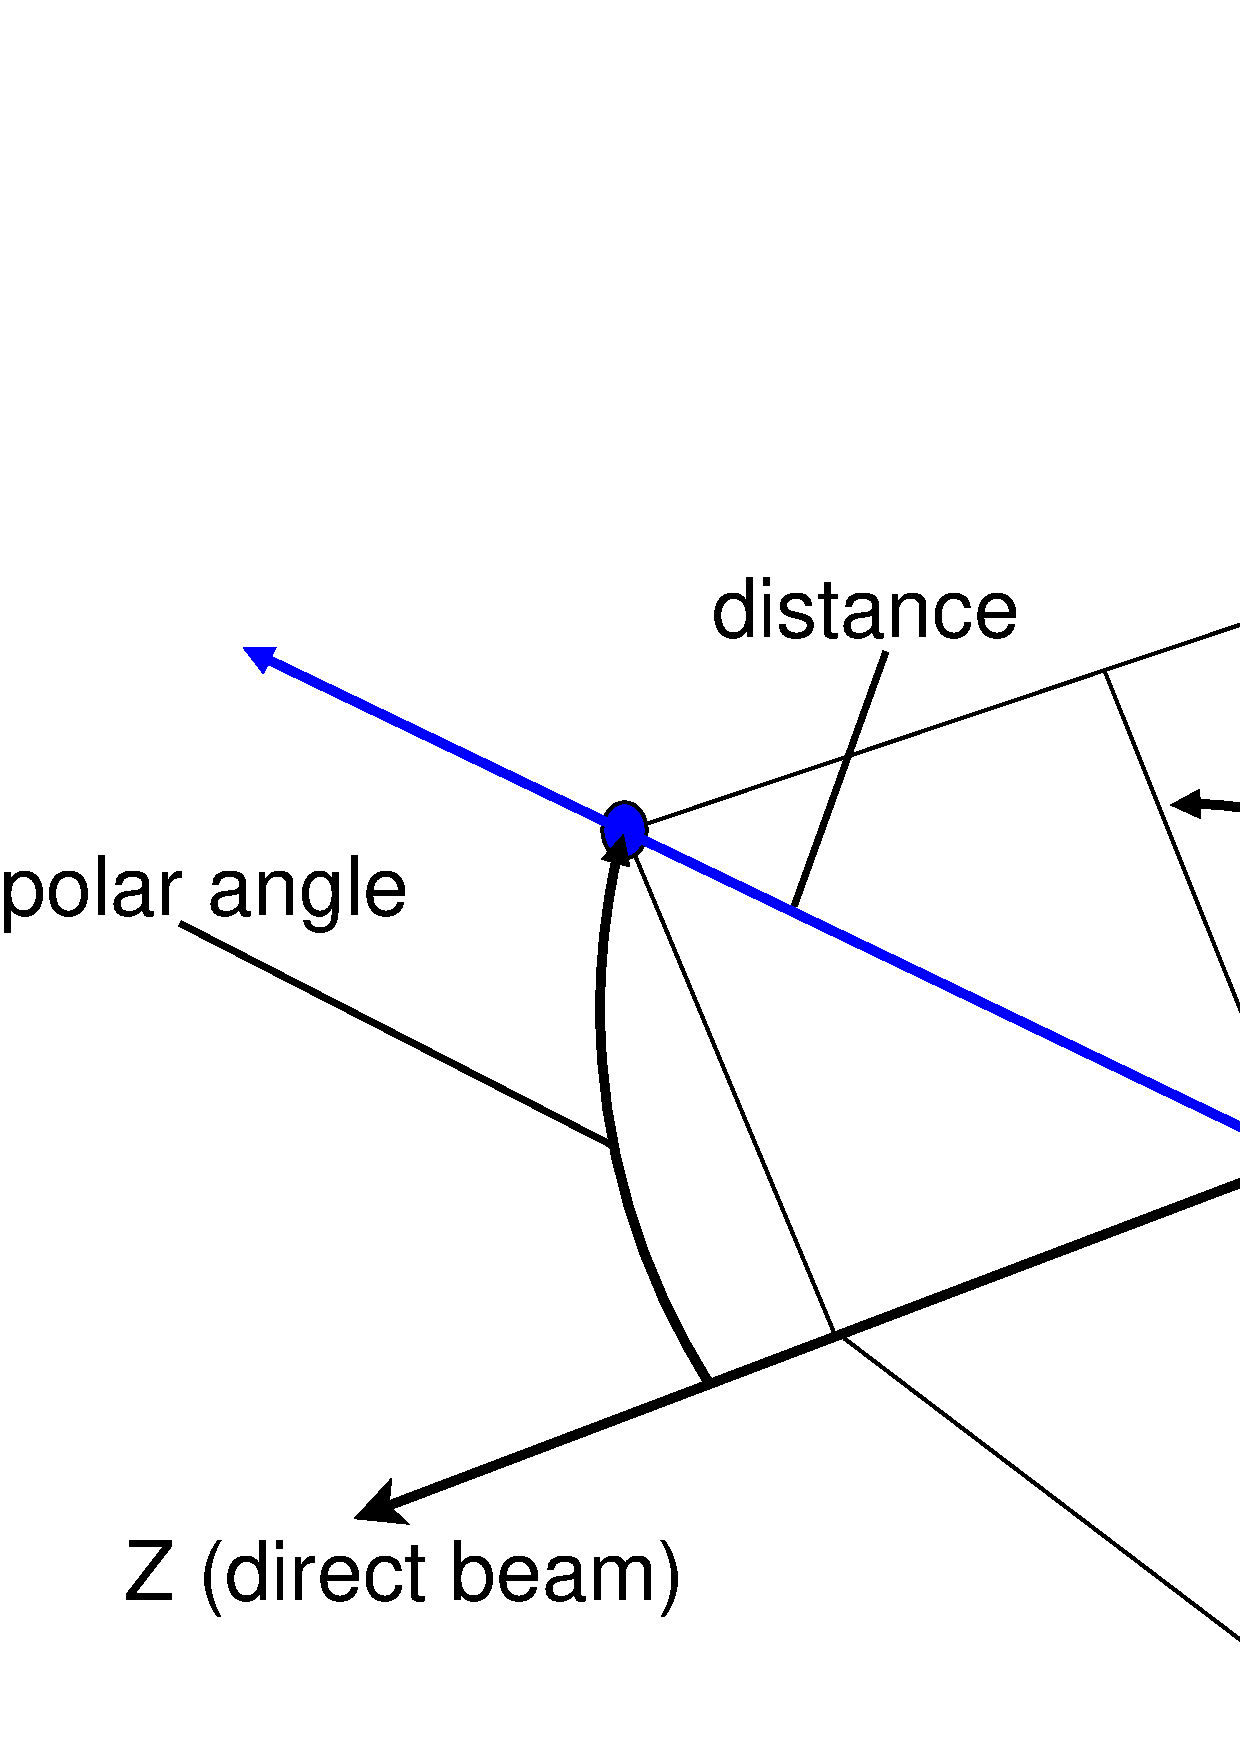
\includegraphics[width=0.75\textwidth]{polplane.png}}\end{figure}
\end{frame}

\begin{frame}
\frametitle{The Predicament of the Traveling Scientist}
\begin{itemize}
\item<1->A different data format wherever she goes
\item<2->Spends lots of time converting formats or writing readers
\item<3->Waits even longer to load data from inefficient data formats
\item<4->DA requires N files in different  formats, notes, local knowledge 
\item<5->Cannot read her collaborators data
\item<6->Has to keep extra information in yet another form
\end{itemize}
\end{frame}
